\documentclass[11pt]{article}
\usepackage[a4paper,left=0.7in,right=0.7in,top=0.6in,bottom=1in]{geometry}
\usepackage{graphicx}
\usepackage{url}
\usepackage{datetime}
\linespread{1.2}

\title{\textbf{Bulldozer Machine Simulation : Project Report} \\ CS296: Software Systems Lab (Group 29)}

\author{
  Shyam JVS\\
  120050052\\
  \texttt{shyam123.jvs95@gmail.com}
  \and
  Soma Naik\\
  120050080\\
  \texttt{somanaik2411@gmail.com}
  \and
  Sumanth Vakulabharanam\\
  120050069\\
  \texttt{sumanthbharan@gmail.com}\\
}
\date{\today}

\begin{document}

\bibliographystyle{plain}
\maketitle

\section{Introduction}

A \textbf{Bulldozer} is a crawler (continuous tracked tractor) equipped
with a substantial metal plate (known as a blade) used to push large quantities of soil, sand, rubble, or other such material during construction or conversion work and typically equipped at the rear with a claw-like device (known as a ripper) to loosen densely compacted materials. \cite{wikipedia} \\
In this project, we have simulated the bulldozer as a complex machine using Box2D\cite{box2d} physics engine. The code for this has been written in C++ making use of the classes/methods provided by Box2D. This simulation has been shown through a GUI created with the help of OpenGL and GLUI open source graphics libraries. Also we have provided with keyboard controls for moving various parts of the bulldozer. \\
This report goes through the details of our project target, the design of the machine, timing measurements on the code, performance of the code measured using gprof (a Linux profiling tool) and ultimately how the profiled statistics helped suggest some code optimizations. 

\section{Design of the machine}

\subsection{Aim and accomplishment}
The image below demonstrates the original design we aimed to make. The key elements that we wanted in the design were - a moving bulldozer on 3 wheels, a belt wrapped around the wheels, a claw-like device at the rear end that could rotate about a hinge and a metal blade at the front end which could both rotate and move up and down. 
\begin{center} 
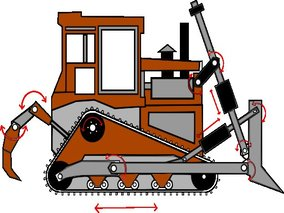
\includegraphics [scale=1.1]{./images/original.jpg} 
\end{center}

\begin{figure}
\centering 
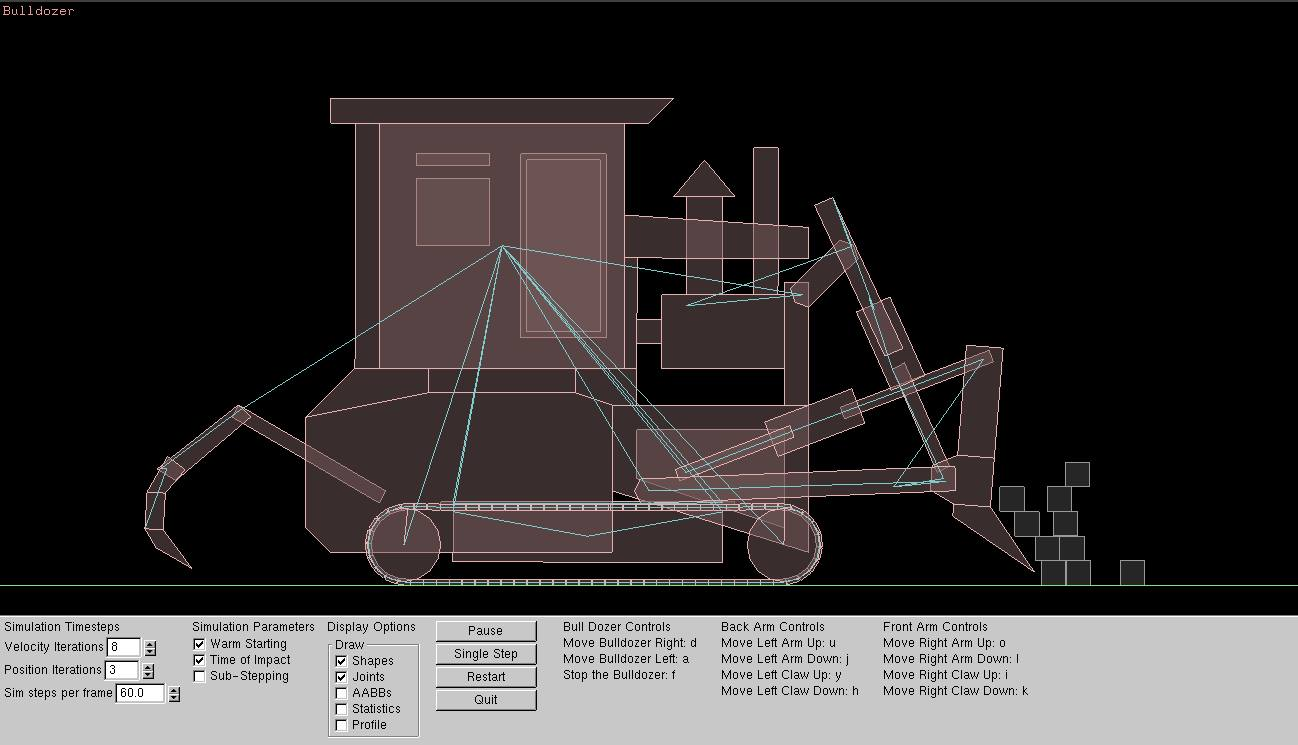
\includegraphics [scale=0.3]{./images/final.jpg} 
\caption{Final Design}
\end{figure}
Above is a screenshot of the final design we have made. We have successfully implemented all the parts we have aimed for - a moving bulldozer on wheels with a chain wrapped around them, the rotatable rear-end ripper with a claw that could be rotated about 2 hinges, the front end metal blade which could be pulled up and down as well as rotated about a hinge. \\
There are a couple of differences between this and the original design. The first being that, instead of using 3 wheels, we have only used 2 wheels in the final design. The reason for doing this is, adding another wheel and hence a longer chain was increasing the number of b2Bodies and revolute joints. Thus on profiling, we found out that there were increased calls to SolveVelocityConstraints(), SolvePositionConstraints() and initVelocityConstraints() methods of class b2RevoluteJoint. To speed up the simulation, we removed the extra wheel and hence the extra chain part as well. The second difference is that, we did not provide too many details about the bulldozer's look (for example a window pane has been removed). This was because, using too many fixtures for the body makes the simulation slow by making too many calls to methods concerning b2PolygonShape and b2Vec2. 

\subsection{Features of our simulation}
Here are the prime elements involved in our design: \\
1. \textbf{Wheel and chain mechanism}: \\
2. \textbf{Motor-driven rear end claw}: \\
3. \textbf{Motor-driven rear end claw}: \\
4. \textbf{Front end blade}: \\
5. \textbf{Suspension rods with variable length}: \\

The following points show the unique features in our design: \\
1. what should be here ?? \\

\section{Analysis of the Timing Diagrams} 

The creation and analysis of timing plots for various attributes involved in computation has been done using 'matplotlib' plotting module\cite{matplotlib} in Python. For the analysis, we varied the number of iterations for which the simulation is carried out from 1 to 200. Also, for each iteration value, the simulation has been rerun for 100 times (just for statistical consistency). The plots that we obtained turned out to be quite interesting. In this section, we present their analysis. \\

\subsubsection{Plot of averaged step time and loop time v/s no. of iterations}
We clearly notice that the avg. loop time increases almost linearly with the no. of iterations.(See plot below) This is quite intuitive, as the number of loops is equal to the iteration value (n) and each iteration takes roughly the same time to finish (as there are just a few floating point operations for carrying out 1 step of the simulation, in each iteration). Hence the loop time is increasing linearly with 'n'. Section 3.2 discusses the variation of Avg. step time.

\begin{center} 
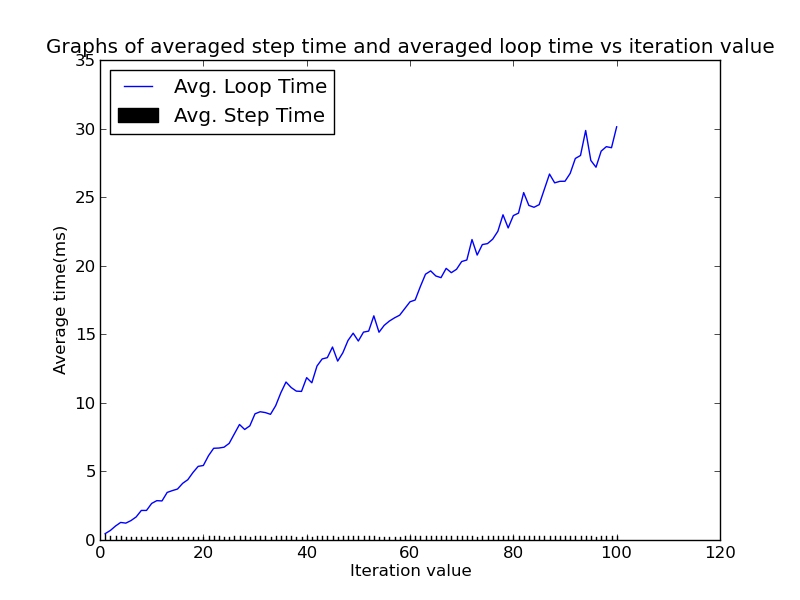
\includegraphics [scale=0.45]{./images/g29_plot01.png} 
\end{center}

\subsubsection{Plot of averaged step time(with Y-error bars) v/s no. of iterations}
Observe that the avg. step time decreases with the value of 'n' initially. (See figure below for the plot along with error bars) Greater values of the step time at the start can be reasoned out using the following logic that, initially the simulation has to adjust and validate the objects' dynamics and other conditions like overlap between rigid bodies, collision at various points etc, which may not be so significant later on. Note that the step time values can show slight ups and downs later on based on the situation of our World. Say if at some point there are many objects close to each other and possibly multiple collissions happening, then the step time may rise for a brief period, and hence increasing (/decreasing) the avg. step time as well. However, what is interesting is that, eventually, after a large number of iterations, the system stabilizes to an almost static state, where most of the bodies either settle down or move at constant rates. At this point the avg. step time becomes almost constant asymptotically.

\begin{center} 
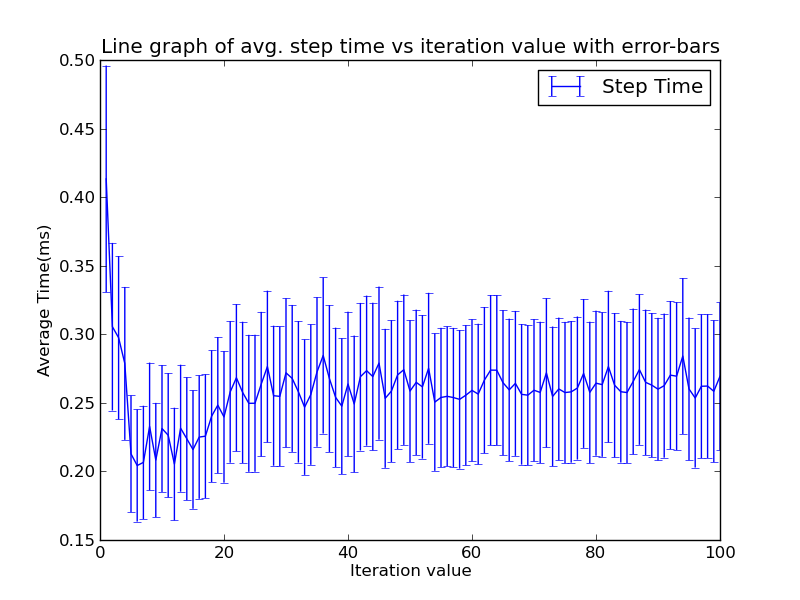
\includegraphics [scale=0.45]{./images/g29_plot03.png} 
\end{center}

\subsubsection{Plot of avg. collision time, velocity and position update times v/s no. of iterations}
Consider the variation of avg. collision time, avg. velocity time and avg. position time with the iteration value. All these 3 variables show a similar variation to that of the avg. step time (see plot below). They remain almost constant with 'n', (with an initial fall due to reasons similar to that for step time) showing that the time taken for these operations is more or less the same for each step. These can slightly vary depending on the situation (similar to step time). Also, it is worth noting that the sum

\begin{center} 
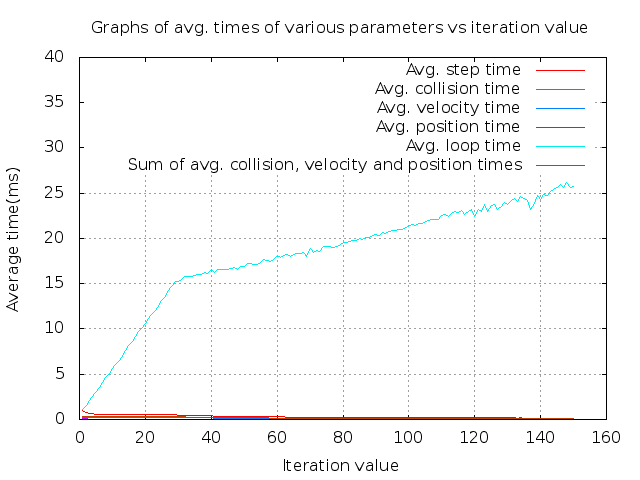
\includegraphics [scale=0.45]{./images/g29_plot02.png} 
\end{center}

\subsubsection{Histogram and Cumulative Frequency Plot of step time}
The figure below shows the histogram plot of step times over the reruns for n = 100. The bars in the plot stand for the relative frequency of step times in that particular bucket. The mean value of step time comes out to be around 0.23ms . And it is evident that most of the frequency is concentrated around the mean, and follows(roughly) a gaussian (bell-shaped) distribution around it. Hence the sampling is statistically consistant as per the central limit theorem. 

\begin{center} 
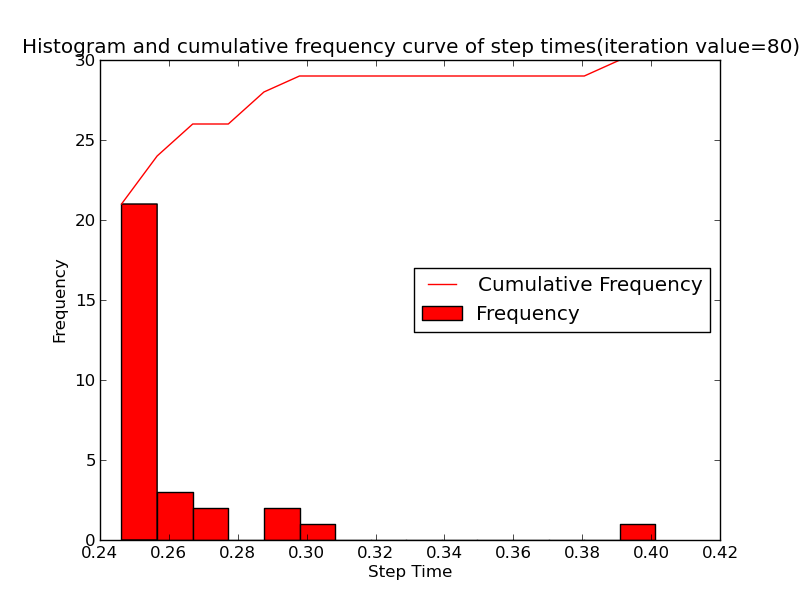
\includegraphics [scale=0.45]{./images/g29_plot04.png} 
\end{center}

\subsection{Performance on a heavily loaded system}
When we ran the base code with n = 20000 while the system was running free (without many heavy processes), it took around 2.890 seconds of running time on an average (measured using the 'time' command in linux). Now the system was loaded with some heavy programs such as libre packages, image viewer, a few memory-consuming and processing-power consuming C++ codes etc. The base code run with the same 'n', now took slightly more time to finish. It took about 2.910 seconds on an average. The increase is clearly due to lesser availability of system resources to the program. 

\subsection{Difference between measurements made using 'time' and 'gettimeofday'}
For n = 20000, avg. time required for execution measured using the 'time' command was around 2896 ms. This accounted for the total real time used by the program (including the standard I/O). However, the total loop time measured by taking the difference of times between the begin and end of the 'for' loop inside the program, using gettimeofday() command is around 2892 ms. This time is slightly less than the one measured by 'time' command because, the 'time' command also includes the time taken by other steps in main.cpp not covered under the loop.\\


\section{Insights from the Profiled Code}

We have used 'gprof' (GNU profiler) as the profiling tool. On profiling the data, we made the call graph. After this, we tried to draw conclusions on the bottleneck parts of our code in terms of time consumed and calls made to different methods. Following this, some optimizations have been suggested.

\subsection{Release Mode}
We have first compiled the Box2D and the other source files in the base code, using the release mode. This included the addition of -O3 flag to the compiler options of g++ and also running cmake on the Box2D package with '-DCMAKE\_BUILD\_TYPE=Release' option. \\
The following was the output of profiling: \\ 

\begin{center} 
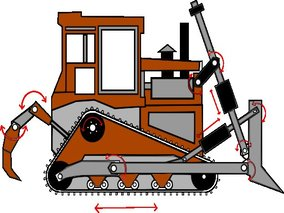
\includegraphics [scale=1.1]{./images/original.jpg} 
\end{center}

We have obtained the call graph for the profile as an image using the 'gprof2dot.py' python script\cite{gprofcode}. This pictorially shows the calling relationships between various subroutines of the base code. The nodes represent functions and also information about the fraction of time taken by them in the total execution time . A directed edge from node 'a' to node 'b' represents the function call to 'b' from 'a'. This edge holds the information about how many times such a call is being made and the percentage of the time spent by calls to 'b' from 'a', out of all calls made from 'a'. \\
The call graph for this mode is shown below: \\
(The graph can't be shown completely, as it is very long. The actual image is at "doc/images/release.png" wrt the project root.)

\begin{center} 

\includegraphics [scale=0.04]{./images/release_100000.png}
\end{center}


\subsection{Debug Mode}
Following the release mode, we again recompiled the Box2D and the other source files in the base code, but this time using the debug mode. This required the exclusion of the -O3 optimization flag from the previous options of g++ and also running cmake on the Box2D package with '-DCMAKE\_BUILD\_TYPE=Debug' option. \\
The following was the output of profiling: \\ 

\begin{center} 
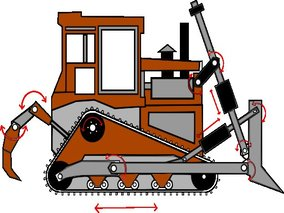
\includegraphics [scale=1.1]{./images/original.jpg} 
\end{center}

The call graph for this mode is shown below: \\
(Again, the graph is long and hence the same problem. The actual image is at "doc/images/debug.png" wrt the project root.)

\begin{center} 
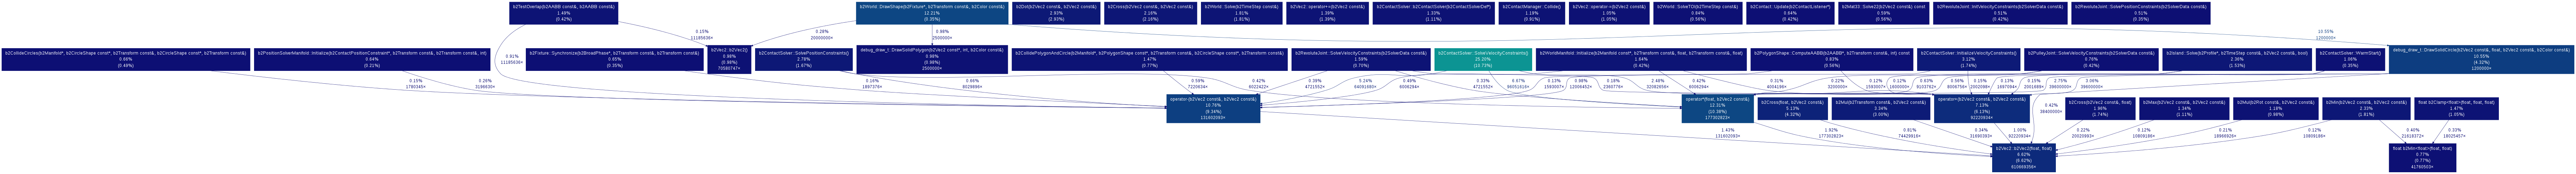
\includegraphics [scale=0.07]{./images/debug_100000.png} 
\end{center}

\subsection{Differences between Debug and Release modes}
Debug and Release are different configurations for building a project. As the name implies, you generally use the Debug mode for debugging your project, and the Release mode for the final build for end users. The Debug mode does not optimize the binary it produces (as optimizations can greatly complicate debugging), and generates additional data to aid debugging. The Release mode enables optimizations and generates less (or no) extra debug data. \\
The -O compiler variable of g++ decides the overall level of optimization. This makes the code compilation take somewhat more time, and can take up much more memory, especially as you increase the level of optimization. 
In the release mode, we have added the -O3 optimization flag, which is the highest level of optimization possible with g++. It turns on optimizations that are expensive in terms of compile time and memory usage. \\
The following are the key observations and differences noted from the profile data generated using the debug and release modes:  \\

1. In release mode, maximum proportion of time is taken by the function \\ b2ContactSolver::SolveVelocityConstraints() which is about 33\%, whereas, in debug mode the same function takes only 10.7\% of the time, though it still remains the most time-consuming. \\

2. In release mode, the function debug\_draw\_t::DrawSolidPolygon(b2Vec2 const*, int, b2Color const\&) is called the maximum number of times (2500000 times)among all functions and consumed about 1.05\% of the total time. Whereas in debug mode, the function b2Vec2::b2Vec2(float, float) is called the maximum number of times (610669356 times) and took 6.62\% of the total time. \\

3. Similarly, we can notice other such functions from the profile data and the call graph, which consume considerable amount of time to get a deeper insight into the functioning of the code. \\

4. It should be noted that, when we run the code with fewer iterations (in the range of 1000-10000) the total loop time is quite fluctuating. To avoid that and obtain stable results, we are using a large number of iterations (= 100000). \\

5. In the release mode, we are using the optimization option -O3 whereas in the debug mode we are not using any optimization options. Hence the total loop time in release mode (2842.357178 ms) is about one-tenth of the total loop time in debug mode (24498.611328 ms), for the same number of iterations. It is therefore clear that this option (-O3) increases the compile time and memory usage but decreases the execution time.


\subsection{Some suggestions for Optimization of the base code}
Most of the time is taken by the function \textbf{b2ContactSolver::SolveVelocityConstraints()} in the Box2D library in both the modes. So if we can optimize this function we can significantly reduce the total loop time. This is one such instance of a possible optimization. We could find more, by a more detailed inspection of the profile data. In general we could say it as a thumb rule that, functions that are called quite frequently or that consume more time should be optimized. Those functions which take almost the same time in both the modes should be focussed upon especially, as the -O3 option is not able to perform much optimization with them.

\end{document}
